\chapter{Layout Languages as Sugared Attribute Grammars}
\section{Motivation and Approach}

We start by examining challenges for building layout languages and our high-level solution of automation through attribute grammars.  Throughout this and the remaining chapters, we focus on the design and implementation of one simple layout widget. We will show how our support of it generalizes to common layout languages and, more generally, computations over trees.

\subsection{Important properties for layout languages and others}
Layout languages are some of the most common -- for one gauge, there are over 634 million websites live in 2012, with 51 million added that year~\footnote{http://news.netcraft.com/archives/2012/12/04/december-2012-web-server-survey.html}. Beyond the CSS and HTML languages used for webpage layout, designers also use \LaTeX~[[CITE]] for document layout, D3~[[CITE]] for data visualization, Swing~[[Swing]] for GUI layout, and even specialize within these domains such as by using markdown for text. 


Popular layout languages foster designer productivity by providing abstractions that are rich and numerous.
The alternative is analogous to asking a programmer to write in a low-level language such as assembly: designers should not manually specify, for each element, the position on a canvas and the style. Instead, layout languages resemble constraint systems where designers  declare high-level properties. For example, the high-level program \code{hello world} states that the words \code{hello} and \code{world} should be rendered, and word \code{world} should follow line-wrapping rules for its positioning after \code{hello}. Layout languages may provide quite complicated constraints -- for example, most document layout languages resort to defining their line wrapping rule  in a flexible low-level language. Likewise, they may provide many featuress, such as in the 250+ pages of rules for the CSS language. Adding to the sophistication, many languages support designers adding their own constraints, such as through macros in \LaTeX,  percentage constraints in CSS, and arbitrary functions in Adobe Flex~[[CITE]]. 

The richness of popular layout languages comes at the cost of of complicating their design and implementation:

\begin{itemize}
\item \textbf{Safe semantics.} Does every input layout have exactly one unique rendering? Are the constraints restricted enough such that an efficient implementation is feasible for low-power devices, big data sets, and fast animation? When a feature is added, does it conflict with anything of the above properties? We want an automated way to verify such properties.
\item \textbf{Safe implementation.} As a layout language grows in popularity, it grows in features. Likewise, developers will port it to many platforms and optimize it, and in cases such as CSS, reimplement it from scratch. Does the implementation conform to the intended semantics? Conformance bugs for CSS plague developers~[[CITE]], and failures to match {\LaTeX}'s semantics have killed multiple attempts to modernize the implementation. We want an automated way to ensure that the implementation matches the specification.
\item \textbf{Advanced implementation.} Layout languages tend to add feature as they evolve. However, the implementation of each feature also has demands that increase with time: improved speed and memory footprint, better debugging support, etc. Browser layout engines for CSS are currently over 100,000 lines of optimized C++ code, and most rich layout languages thus far have resisted parallelization. We want automation techniques to lower the implementation burden and more aggressively target those goals.
\end{itemize}


\begin{figure}
\centering
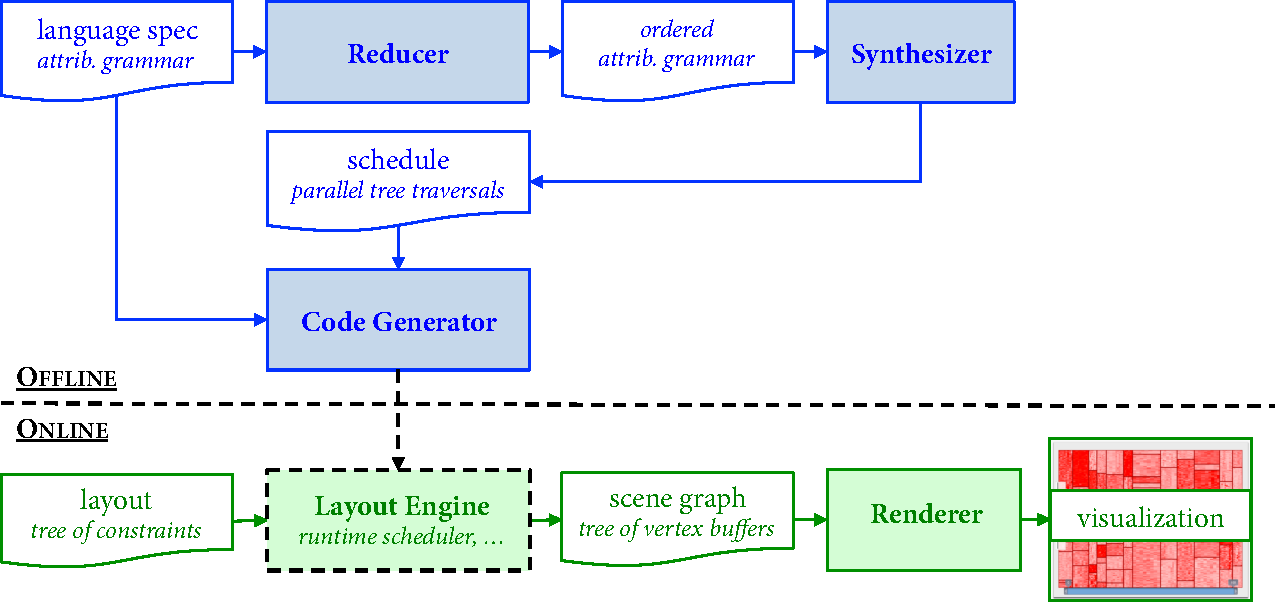
\includegraphics[trim=0 0 0 0,clip,width=1.0\columnwidth]{chapter2/architecture}
\caption{\textbf{Layout engine architecture.} }
\label{fig:architecture}
\end{figure}

Our idea is to declaratively specify layout languages and automatically compile them into an efficient implementation. At runtime, an instance of layout will be processed through the previously generated layout engine (Figure~\ref{fig:architecture}). The compiler is responsible for checking the semantics of the layout features and, by construction, provides a correct implementation. Furthermore, instead of manually optimizing the code for every individual feature, language designers instead write generic compiler optimizations. As a similar implementation benefit, we automatically target multiple platforms for the same layout language, such as scripting languages in order to use their debuggers, and multicore and GPU languages to gain magnitudes of speedups.

We show that the attribute grammar formalism supports specification of layout languages. It is unclear how to encode complicated layout language features with the traditional formalism, so we support a rich form of attribute grammars and reduce reasoning about them to handling a more traditional formalism (reducer in Figure~\ref{fig:architecture}). The remainder of this chapter introduces the high-level attribute grammar formalism, how to specify layout languages using it, and an intuition for the reduction into a lower-level formalism.


\newsavebox{\agdef}
\begin{lrbox}{\agdef}% Store first listing
\begin{minipage}{1\columnwidth}
\setlength{\grammarparsep}{0.15cm}   % vertical distance between production rules
\setlength{\grammarindent}{1cm}
\renewcommand{\litleft}{\bfseries}
\renewcommand{\ulitleft}{\bfseries}
\renewcommand{\superscript}[1]{\ensuremath{^{\textrm{#1}}}}
\renewcommand{\subscript}[1]{\ensuremath{_{\textrm{\uppercase{#1}}}}}
\renewcommand{\syntleft}{\normalfont\itshape}
\renewcommand{\syntright}{}
%\newcommand{\deriv}{~::=~}
\renewcommand{\deriv}{~ $\rightarrow$ ~}
\begin{grammar}
<AG> \deriv{} (<Prod> "\{" <Stmnt>? "\}")*

<Prod> \deriv{} <V> $\rightarrow$ <V>*

<Stmnt> \deriv{} <Attrib> "=" <id>(<Attrib>*) ~  | ~ <Attrib> "=" <n> ~ | ~ <Stmnt> ; <Stmnt> 

<Attrib> \deriv{} <id>.<id>
\end{grammar}
\end{minipage}
\end{lrbox}



\newsavebox{\hboxtreetext}
\begin{lrbox}{\hboxtreetext}% Store first listing
\begin{lstlisting}[language=C++,morekeywords={spawn,join,reverse,parallel_for}]
<S>
  <HBox>
    <HBox>
      <HBox w=20 h=5/>
      <HBox w=15 h=5/>
    </HBox>
    <HBox w=15 h=5/>
  </HBox>
</S>
\end{lstlisting}
\end{lrbox}


\begin{figure}
\subfloat[\textbf{Input tree.} Only some of the x, y, w, and h attributes are specified.]{\label{fig:hbox:input}
\begin{minipage}{1\columnwidth}\centering
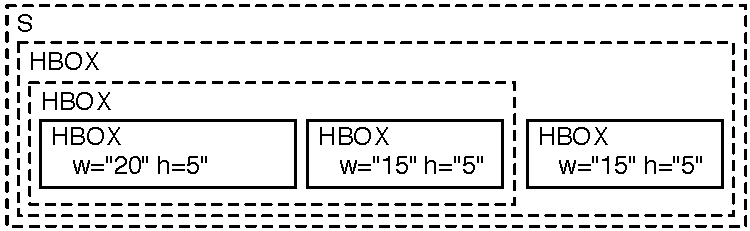
\includegraphics[trim=0 0 0 0,clip,width=1.0\columnwidth]{chapter2/output}
\end{minipage}}\\
\subfloat[\textbf{Textual encoding of input tree.}]{\label{fig:hbox:texttree}
\begin{minipage}{1\columnwidth}\centering
\usebox{\hboxtreetext}
\end{minipage}
}\\
\subfloat[\textbf{Attribute grammar for a language of horizontal boxes.}]{\label{fig:hbox:grammar}
\begin{minipage}{1\columnwidth}
\begin{grammar}
<S> \deriv{} \emph{HBOX} \\ 
  \{ HBOX.x = 0; HBOX.y = 0 \}

<HBOX> $\rightarrow$ $\epsilon$  \\
\{ HBOX.w = input$_w$(); HBOX.h = input$_h$() \} 

<HBOX$_0$> $\rightarrow$ \emph{HBOX$_1$} \emph{HBOX$_2$} \\
\{ HBOX$_1$.x = HBOX$_0$.x; \\
$~~~$ HBOX$_2$.x = HBOX$_0$.x + HBOX$_1$.w; \\
$~~~$ HBOX$_1$.y = HBOX$_0$.y; \\
$~~~$ HBOX$_2$.y = HBOX$_0$.y; \\
$~~~$ HBOX$_0$.h = max(HBOX$_1$.h, HBOX$_2$.h); \\
$~~~$ HBOX$_0$.w = HBOX$_1$.w + HBOX$_2$.w \} 
\end{grammar}
\end{minipage}
}\\
\subfloat[\textbf{Language of attribute grammars.}]{\label{fig:ag}
\usebox{\agdef}
}
\caption{For a language of horizontal boxes: (a) input tree to solve and (b) attribute grammar specifying the layout language. Specification language of attribute grammars shown in (c).%and (c) dynamic data dependencies.
}
\label{fig:hbox}
\end{figure}


\section{The HBox Language as a Classical Attribute Grammar}

This section describes specifying a simple layout language as an attribute grammar and two classical implementation strategies. We reuse the example throughout our work to explore various concepts.



\subsection{Attribute Grammars}

Consider solving the tree of horizontal boxes shown in Figure~\frefb{fig:hbox}{fig:hbox:input}. As input, a webpage author provides a tree with constraints (Figure~\frefb{fig:hbox}{fig:hbox:text tree}). Only some node attribute values are provided: in this case, only the widths and heights of leaf nodes. The meaning of a horizontal layout is that, as is visualized, the boxes will be placed side-by-side. The layout engine must solve for all remaining x, y, width, and height attributes. 

We declaratively specify the layout language of horizontal boxes, \hlang{},  as shown in Figure~\frefb{fig:hbox}{fig:hbox:grammar}, with an attribute grammar~\cite{oag,Meyerovich:2010,htmlag}. First, the specification defines the set of well-formed input trees as the derivations of a context-free grammar. We use the standard notation~[[CITE]]. In this case, a document is an unbalanced binary tree of arbitrary depth where the root node has label \texttt{S} and intermediate nodes have label \texttt{HBOX}. Second, the specification defines semantic functions that relate attributes associated with each node. For example, the width of an intermediate horizontal node is the sum of its children widths. Likewise, the width of a leaf node is provided by the user, which is encoded by the nullary function call $input_w()$:


\begin{grammar}
<HBOX> $\rightarrow$ $\epsilon$ \{ HBOX.w = $input_w$(); $\ldots$ \} ~~~~~~~~~~~~~~~~~~~~~~~ /* leaf */

<HBOX$_0$> $\rightarrow$ \emph{HBOX$_1$} \emph{HBOX$_2$} ~~~~~~~~~~~~~~~~~~~~~~~~~~~~~~~~~ /* binary node */\\
\{ $\ldots$ HBOX$_0$.w = HBOX$_1$.w + HBOX$_2$.w \} 
\end{grammar}


The specification intentionally does not define the evaluation order. For example, the specification does not state whether to compute a node's width before its height. Likewise, our optimized approach will compute the attributes as a sequence of tree traversals, but the specification does not state what those traversals are. Leaving the evaluation order unspecified provides freedom for our compilers to pick an efficient parallel order. Irrespective of whatever evaluation order is ultimately used to solve for the attribute values, the statements define constraints that must hold over the computed result. Attribute grammars can therefore be thought of as a single assignment language where attributes are dataflow variables~[[CITE]].
zzz

The language of attribute grammars is defined in Figure~\frefb{fig:hbox}{fig:ag}. 
Our example assumes the following encoding. Semantic functions are pure and left uninterpreted, so, for example, we encode the addition of widths as ``\mbox{HBOX$_0$.w = f(HBOX$_1$.w, HBOX$_2$.w)}''. Likewise, constant values are equivalent to nullary function calls. Our program analysis techniques do not need to know the contents of the function, just that the output of a call depends purely on the inputs. 

To specify grammars more complicated than \hlang{}, we describe linguistic extensions for richer functional specifications (Section~\ref{sec:desugaring}) and, to control the evaluation order, behavioral specification (Chapters~\ref{chap:3} and \ref{chap:4}).

\begin{figure}
\centering
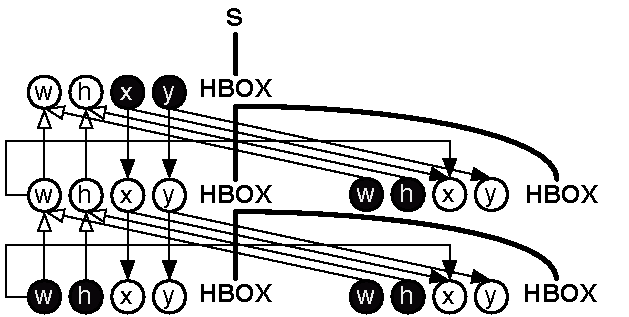
\includegraphics[trim=0 0 0 0,clip,width=0.8\columnwidth]{chapter2/deps}
\caption{\textbf{Data dependencies.} Shown for constraint tree  in Figure~ZZZ~(a). Circles denote attributes, with black circles being \sched{input()} sources. Thin lines show data dependencies and thick lines show production derivations.}
\label{fig:deps}
\end{figure}

\subsection{Dynamic data dependencies and dynamic evaluation}


\subsection{Static data dependencies and static evaluators}


\section{Desugaring Loops and Other Modern Constructs}
\label{sec:desugaring}
\subsection{Motivation: Productive Features with Simple Implementations}
\subsection{Interfaces: Lightweight and Reusable Input/Output Specifications}
\subsection{Traits: Reusing Cross-cutting Code}
\subsection{Loops}
\subsection{Embedded Domain Specific Language: Functional Rendering}



\section{Evaluation: Mechanized Layout Features}





\subsection{Rendering: Immediate Mode and Beyond}
\subsection{Non-euclidean: Sunburst Diagram}
\subsection{Charts: Line graphs}
\subsection{Animation and Interaction: Treemap}
\subsection{Flow-based: CSS Box Model}
\subsection{Grid-based: HTML Tables}

\section{Related Work}
\begin{itemize}
\item loose formalisms: browser impl (C++), d3 (JavaScript), latex formulas (ML)
\item restricted formalisms: cassowary and hp, UREs
\item AGs: html tables
\end{itemize}



